\documentclass[12pt]{article}
\newcommand{\gradeband}{Grades K–1}
% Shared layout for the Week 7 student pages (compile with xelatex)
\usepackage[letterpaper, top=0.95in, bottom=0.75in, left=0.8in, right=0.8in,
            headheight=20pt, headsep=16pt, footskip=28pt]{geometry}
\usepackage{fontspec}
\setmainfont{Andika}
\usepackage{xcolor}
\usepackage{tikz}
\usetikzlibrary{arrows.meta,positioning,calc}
\usepackage[most]{tcolorbox}
\usepackage{fancyhdr}

\pagestyle{fancy}
\fancyhf{}
\lhead{\small Bellingham Math Circle \enspace\textperiodcentered\enspace Week 7
       \enspace\textperiodcentered\enspace \gradeband}
\rhead{\small Name \rule[-2pt]{5cm}{0.5pt}}
\cfoot{\small \thepage}
\renewcommand{\headrulewidth}{0.4pt}

\setlength{\parindent}{0pt}
\setlength{\parskip}{5pt}
\hyphenpenalty=10000
\exhyphenpenalty=10000
\AtBeginDocument{\raggedright}

\newcounter{prob}
\newcommand{\problem}{\stepcounter{prob}\par\textbf{Problem \theprob:}\enspace}

\newtcolorbox{rulebox}{enhanced, colback=white, colframe=black!55,
  boxrule=0.7pt, arc=2mm, left=8pt, right=8pt, top=6pt, bottom=6pt,
  before upper=\raggedright}

% ---- counters -------------------------------------------------------------
\tikzset{
  ctr/.style={circle, draw=black, fill=black!18, line width=0.6pt,
              minimum size=#1, inner sep=0pt},
  ctr/.default=5mm,
  xmark/.style={line width=1.4pt, line cap=round},
  ansbox/.style={draw=black, line width=0.6pt, minimum size=#1, inner sep=0pt},
  ansbox/.default=9mm,
}
% \pile[size]{n}{crossed}{per row}{step}  (drawn with top-left counter at origin)
\newcommand{\pile}[5][5mm]{%
  \foreach \i in {1,...,#2} {%
    \pgfmathtruncatemacro{\col}{mod(\i-1,#4)}%
    \pgfmathtruncatemacro{\row}{(\i-1)/#4}%
    \node[ctr=#1] (p\i) at (\col*#5, -\row*#5) {};%
    \pgfmathtruncatemacro{\thr}{#2-#3}%
    \ifnum\i>\thr
      \draw[xmark] ($(p\i)+(-0.62*#1,0.62*#1)$) -- ($(p\i)+(0.62*#1,-0.62*#1)$)
                   ($(p\i)+(0.62*#1,0.62*#1)$) -- ($(p\i)+(-0.62*#1,-0.62*#1)$);
    \fi
  }}


% one cell of a trap strip: \trapcell{x}{y}{n}
\newcommand{\trapcell}[3]{%
  \begin{scope}[shift={(#1,#2)}]
    \draw[rounded corners=2mm, line width=0.6pt] (0,0) rectangle (2.7,-3.5);
    \node[font=\bfseries\huge, text height=1.6ex, text depth=0.2ex] at (1.35,-0.65) {#3};
    \begin{scope}[shift={(0.35,-1.6)}]
      \pile[4.4mm]{#3}{0}{5}{0.5}
    \end{scope}
    \node[ansbox=10mm] at (1.35,-4.2) {};
  \end{scope}}
\newcommand{\trapstrip}{%
  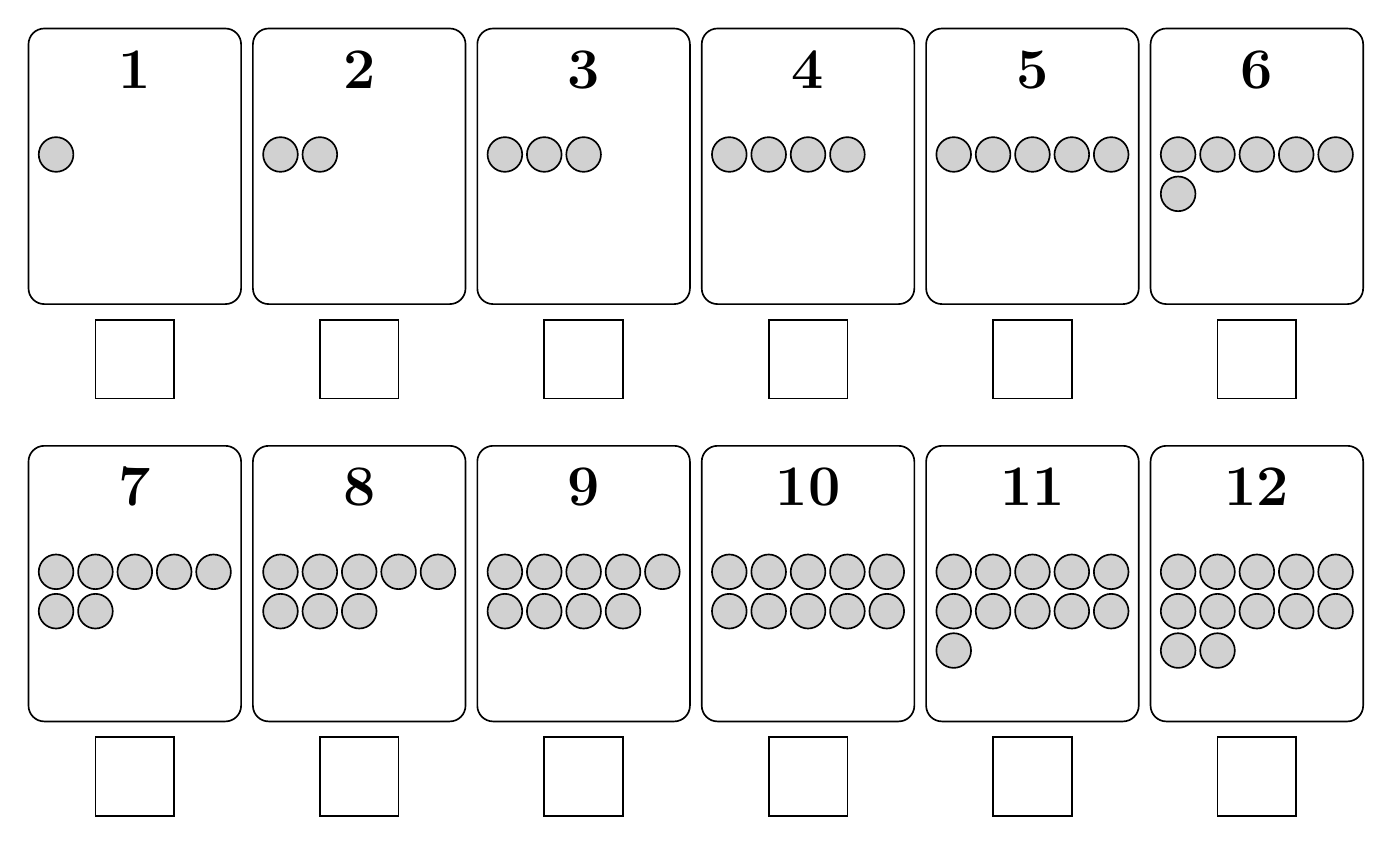
\begin{tikzpicture}
    \foreach \n in {1,...,12} {
      \pgfmathsetmacro{\cx}{mod(\n-1,6)*2.85}
      \pgfmathsetmacro{\cy}{-5.3*int((\n-1)/6)}
      \trapcell{\cx}{\cy}{\n}
    }
  \end{tikzpicture}}

% two piles inside outlines: \twopiles{a}{b}  (at most 5 counters per pile)
\newcommand{\twopiles}[2]{%
  \begin{tikzpicture}[baseline={(0,0.4)}]
    \draw[rounded corners=3mm, line width=0.6pt, black!60] (0,0) rectangle (4.2,1.1);
    \begin{scope}[shift={({(4.2-(#1-1)*0.7)/2},0.55)}]\pile[5.5mm]{#1}{0}{5}{0.7}\end{scope}
    \draw[rounded corners=3mm, line width=0.6pt, black!60] (4.8,0) rectangle (9.0,1.1);
    \begin{scope}[shift={({4.8+(4.2-(#2-1)*0.7)/2},0.55)}]\pile[5.5mm]{#2}{0}{5}{0.7}\end{scope}
  \end{tikzpicture}}

\newcommand{\choice}[1]{\tikz[baseline=(t.base)]\node[draw, rounded corners=2mm,
  line width=0.6pt, inner xsep=10pt, inner ysep=6pt] (t) {#1};}

\begin{document}
\fontsize{15}{21}\selectfont
\setlength{\parskip}{7pt}

\begin{rulebox}
Two players share one pile of counters. They take turns.
On your turn, take away 1 counter or 2 counters.
Whoever takes the last counter wins.

\medskip
\centering
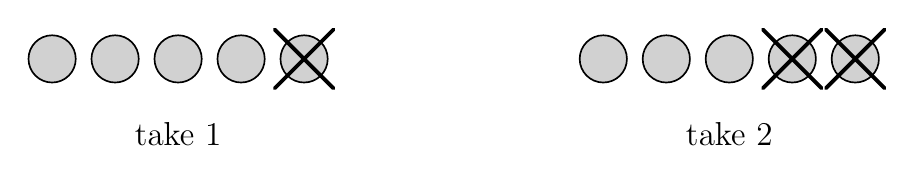
\begin{tikzpicture}
  \begin{scope}\pile[6mm]{5}{1}{5}{0.8}\end{scope}
  \node[font=\large] at (1.6,-0.95) {take 1};
  \begin{scope}[shift={(7,0)}]\pile[6mm]{5}{2}{5}{0.8}\end{scope}
  \node[font=\large] at (8.6,-0.95) {take 2};
\end{tikzpicture}
\end{rulebox}

\bigskip
\problem It is your turn. Can you take the last counter on this turn?
Circle yes or no under each pile.

\medskip
\begin{center}
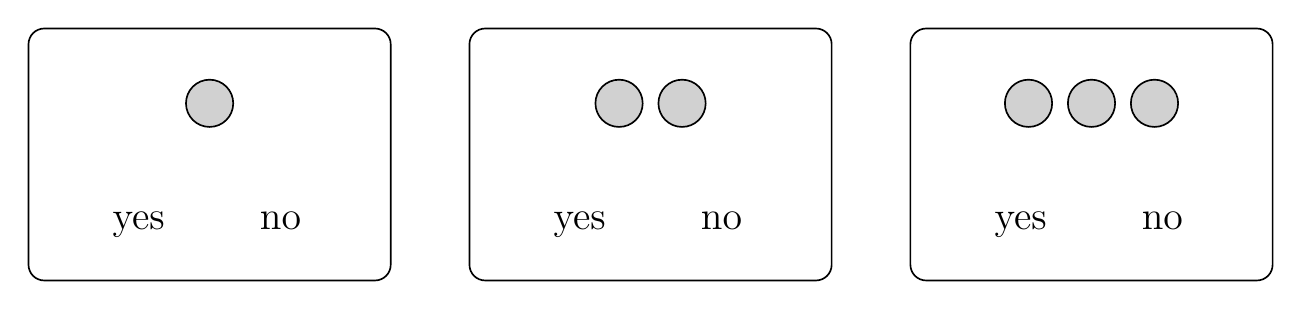
\begin{tikzpicture}
  \foreach \n/\x in {1/0, 2/5.6, 3/11.2} {
    \begin{scope}[shift={(\x,0)}]
      \draw[rounded corners=2mm, line width=0.6pt] (0,0.2) rectangle (4.6,-3.0);
      \begin{scope}[shift={({2.3-0.4*(\n-1)},-0.75)}]\pile[6mm]{\n}{0}{5}{0.8}\end{scope}
      \node[font=\Large, anchor=base] at (1.4,-2.35) {yes};
      \node[font=\Large, anchor=base] at (3.2,-2.35) {no};
    \end{scope}
  }
\end{tikzpicture}
\end{center}

\vspace{1.2cm}
\problem There are 3 counters, and it is your turn. Your partner always plays
carefully. Can you be the player who takes the last counter? Circle yes or no.

\medskip
\begin{center}
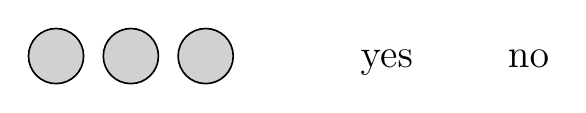
\begin{tikzpicture}
  \begin{scope}\pile[7mm]{3}{0}{5}{0.95}\end{scope}
  \node[font=\Large, anchor=base] at (4.2,-0.15) {yes};
  \node[font=\Large, anchor=base] at (6.0,-0.15) {no};
\end{tikzpicture}
\end{center}

\vfill
\newpage

\begin{rulebox}
A pile is a \textbf{trap} when the player whose turn it is will lose
if the other player plays carefully.
\end{rulebox}

\medskip

\problem Which of these piles are traps? Draw an X in the box under each trap.

\medskip
\begin{center}
\trapstrip
\end{center}

\vfill
\newpage

\problem There are 6 counters, and it is your partner's turn. Your partner
might take 1 or might take 2. For each choice, write how many counters you
will take next so that you are sure to win.

\medskip
\begin{center}
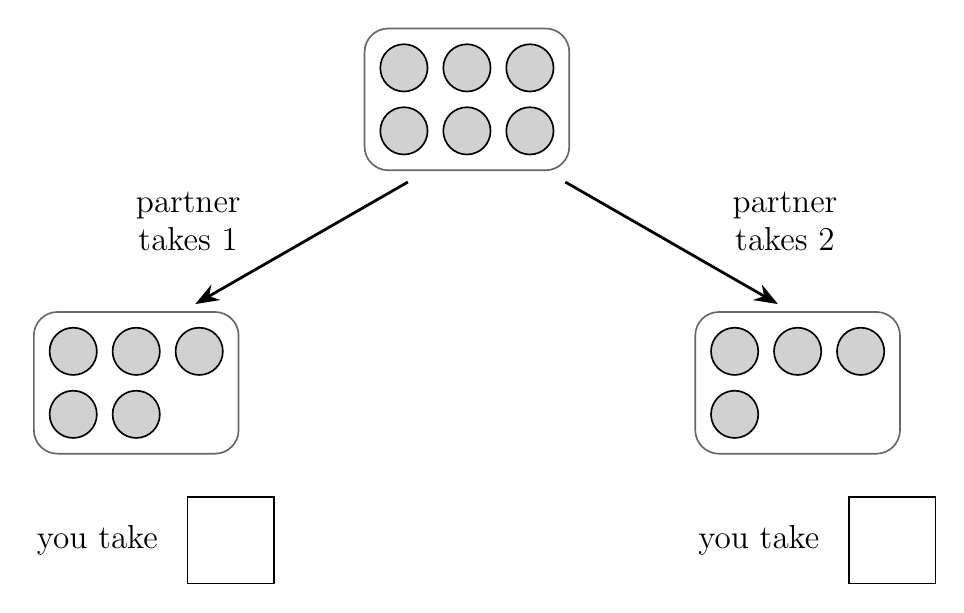
\begin{tikzpicture}[>={Stealth[length=3mm]}]
  % top pile
  \begin{scope}[shift={(4.95,0)}]\pile[6mm]{6}{0}{3}{0.8}\end{scope}
  \draw[rounded corners=3mm, line width=0.6pt, black!60] (4.45,0.5) rectangle (7.05,-1.3);
  % branches
  \draw[->, line width=1pt] (5.0,-1.45) -- (2.3,-3.0);
  \draw[->, line width=1pt] (7.0,-1.45) -- (9.7,-3.0);
  \node[font=\large, align=center, anchor=east] at (3.0,-1.95) {partner\\takes 1};
  \node[font=\large, align=center, anchor=west] at (9.0,-1.95) {partner\\takes 2};
  % left result: 5
  \begin{scope}[shift={(0.75,-3.6)}]\pile[6mm]{5}{0}{3}{0.8}\end{scope}
  \draw[rounded corners=3mm, line width=0.6pt, black!60] (0.25,-3.1) rectangle (2.85,-4.9);
  % right result: 4
  \begin{scope}[shift={(9.15,-3.6)}]\pile[6mm]{4}{0}{3}{0.8}\end{scope}
  \draw[rounded corners=3mm, line width=0.6pt, black!60] (8.65,-3.1) rectangle (11.25,-4.9);
  % answer boxes
  \node[font=\large, anchor=east] at (1.95,-6.0) {you take};
  \node[ansbox=11mm] at (2.75,-6.0) {};
  \node[font=\large, anchor=east] at (10.35,-6.0) {you take};
  \node[ansbox=11mm] at (11.15,-6.0) {};
\end{tikzpicture}
\end{center}

\vspace{1.4cm}
\problem This game started with 8 counters. Each row shows one turn, and the
crossed-out counters are the ones taken on that turn. The first player lost.
Circle the row where the first player could have taken a different number of
counters and then been sure to win.

\medskip
\begin{center}
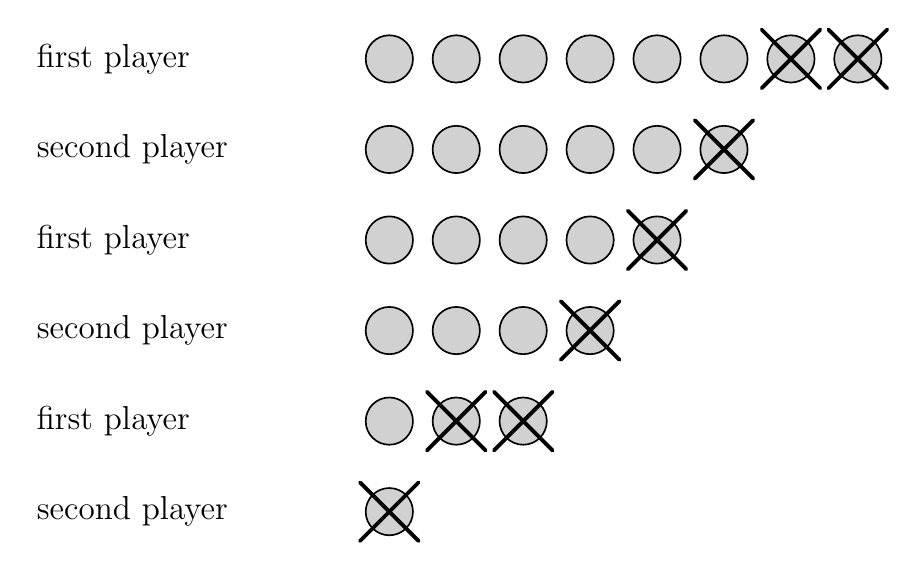
\begin{tikzpicture}
  \foreach \who/\n/\k [count=\r] in
      {first player/8/2, second player/6/1, first player/5/1,
       second player/4/1, first player/3/2, second player/1/1} {
    \begin{scope}[shift={(0,-1.15*\r)}]
      \node[font=\large, anchor=west] at (0,0) {\who};
      \begin{scope}[shift={(4.6,0)}]\pile[6mm]{\n}{\k}{8}{0.85}\end{scope}
    \end{scope}
  }
\end{tikzpicture}
\end{center}

\vfill
\newpage

\problem You will play against the adult at your table with a pile of
9 counters. Before you start, you choose who goes first. Circle the choice
that lets you win, however the adult plays.

\medskip
\begin{center}
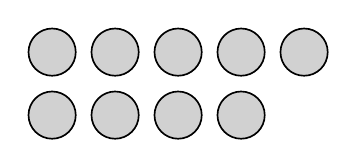
\begin{tikzpicture}
  \begin{scope}\pile[6mm]{9}{0}{5}{0.8}\end{scope}
\end{tikzpicture}

\bigskip
\choice{I go first}\hspace{2cm}\choice{The adult goes first}
\end{center}

\vspace{1.6cm}
\problem Find a trap with more than 12 counters and a trap with more than
20 counters. Draw each one or write its number in a box.

\medskip
\begin{center}
\begin{tikzpicture}
  \draw[rounded corners=3mm, line width=0.7pt] (0,0) rectangle (8,-8.2);
  \node[font=\large, anchor=north west] at (0.2,-0.15) {more than 12};
  \draw[rounded corners=3mm, line width=0.7pt] (8.6,0) rectangle (16.6,-8.2);
  \node[font=\large, anchor=north west] at (8.8,-0.15) {more than 20};
\end{tikzpicture}
\end{center}

\vfill
\newpage

\problem Play with a different rule: on your turn, take away 1, 2, or 3 counters. Whoever takes
the last counter wins. Which piles are traps now? Draw an X in the box under
each trap.

\medskip
\begin{center}
\trapstrip
\end{center}

\vfill
\newpage

\problem Now there are two piles. On your turn, choose one pile and take 1 or
2 counters from that pile only. Whoever takes the last counter wins. For each
game, circle whether you would rather go first or go second.

\medskip
\begin{center}
\renewcommand{\arraystretch}{1}
\begin{tabular}{@{}l@{\hspace{1.2cm}}c@{\hspace{0.7cm}}c@{}}
\twopiles{2}{2} & \choice{go first} & \choice{go second} \\[2.1cm]
\twopiles{2}{1} & \choice{go first} & \choice{go second} \\[2.1cm]
\twopiles{5}{5} & \choice{go first} & \choice{go second} \\[2.1cm]
\twopiles{4}{1} & \choice{go first} & \choice{go second} \\[2.1cm]
\twopiles{3}{1} & \choice{go first} & \choice{go second} \\
\end{tabular}
\end{center}

\vfill
\end{document}
